\chapter{Background knowledge}

\label{ch:Background knowledge}

\setlength{\parindent}{4em}
\setlength{\parskip}{1em}
\renewcommand{\baselinestretch}{1.5}

\section{Background knowledge}

\subsection {Electroencephalography (EEG)}

\hspace{1.5cm} EEG is a technique for studying the electrical activities within the brain using electrodes that attached to the surface of scalp. Wires attach these electrodes to a machine, which records the electrical impulses. The results are either printed out or displayed on a computer screen. Different pattern of electrical impulses can denote various form of epilepsy\cite{ref9}. It is also used to diagnose sleep disorders, coma, encephalopathies, and brain death.\par
Derivatives of the EEG technique include evoked potentials (EP), which involves averaging the EEG activity time-locked to the presentation of a stimulus of some sort (visual, somatosensory, or auditory). Event-related potentials (ERPs) refers to averaged EEG responses that are time-locked to more complex processing of stimuli.

\begin{figure}[h]
	\centering
	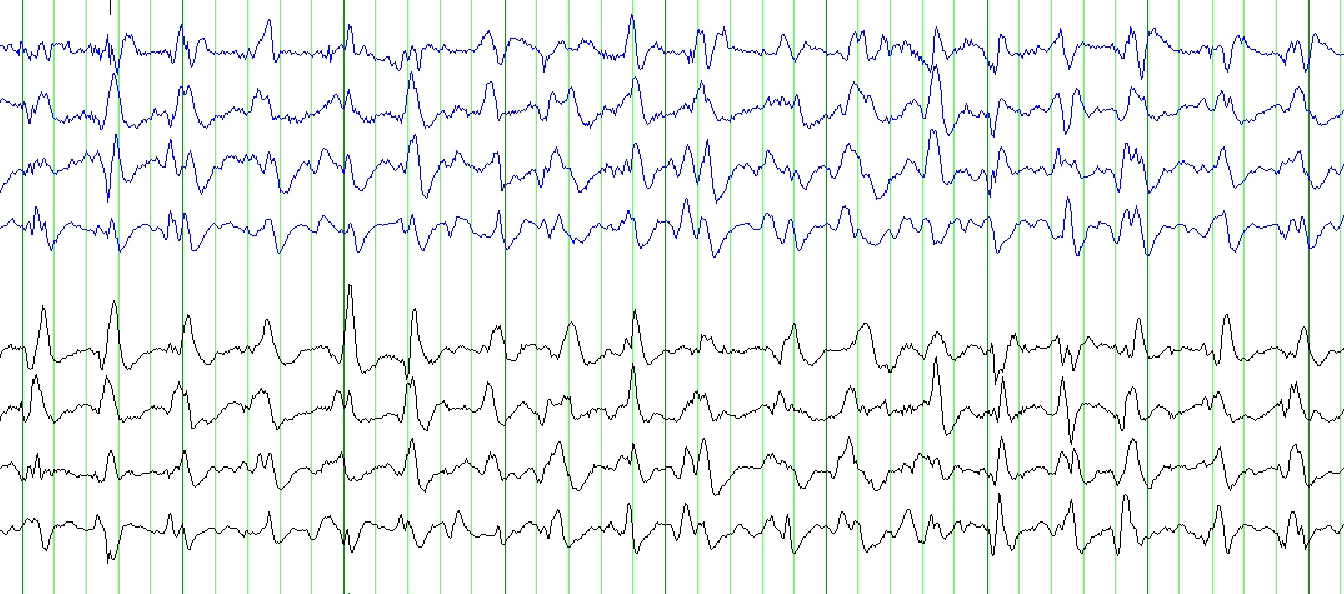
\includegraphics[scale = 0.5]{chapter3/31.pdf}
	\caption{EEG signal}
\end{figure}
\newpage

\subsection{Event-related potential (ERPs)}

\hspace{1.5cm} Event-related potentials (ERPs) are very small voltages generated in the brain structures in response to specific events or stimuli. They measure brain response that is directed result of a specific sensory, cognitive or motor event. To see the brain's response to a stimulus, the experimenter must conduct many trials (usually in the order of 100 or more) and average the results together, causing random brain activity to be averaged out and the relevant waveform to remain, these stimuli can be visual, auditory, tactile and even olfactory and gustatory.

\begin{figure}[h]
	\centering
	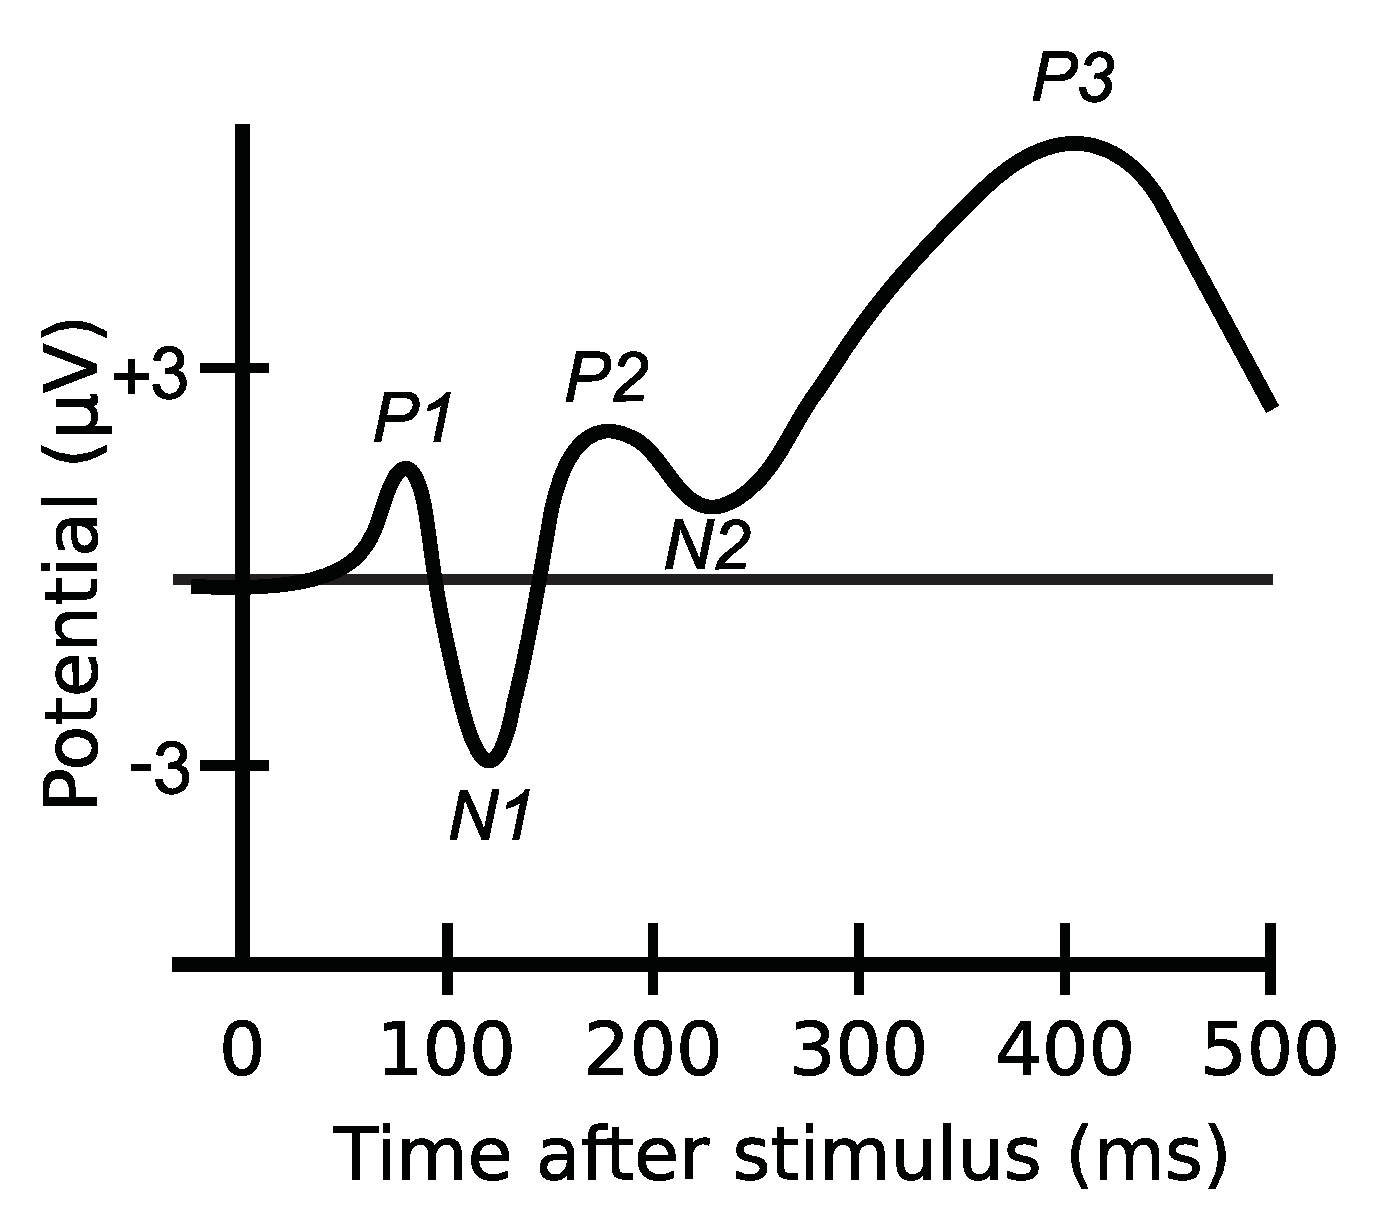
\includegraphics[scale = 0.3]{chapter3/32.pdf}
	\caption{Averaged ERP waveform}
\end{figure}

\newpage
\subsection{Steady state visually evoked potential (SSVEP)}

\hspace{1.5cm} Steady State Visually Evoked Potentials or SSVEPs are signals that are natural responses to visual stimulation at specific frequencies. When the retina is stimulated by a visual stimulus ranging from 3.5 Hz to 75 Hz, the brain generates electrical activity at the same (or multiples of) frequency of the visual stimulus. SSVEP is the EEG signal but we called SSVEP because when the subject is in meditation state the brain will generate a stable EEG waveform but when the subject fixates the visual stimuli the EEG waveform is changing and become SSVEP at that time.\par


\subsection{Cerebral Cortex}

\hspace{1.5cm} The human brain consists of several parts. The part that make human more intelligent than any animals are Cerebrum. Cerebrum is the largest part of human brain. The physician divides the cerebrum into four parts. There is frontal lobe, parietal lobe, temporal lobe and occipital lobe. Frontal lobe is located at the front of the brain. It controls the creative thought, thinking, problem solving and muscle movements. Parietal lobe is positioned above the occipital lobe and behind the frontal lobe. It involved in the visual functions, languages, reading and sensory controls. Temporal lobe situates beneath both frontal lobe and parietal lobe. It implicates in control memories, speech and hearing languages. Occipital lobe related with a human vision controls. Due to our project study about the human visualization, so we focus on the occipital lobe.

\begin{figure}[h]
	\centering
	\includegraphics[scale = 0.32]{chapter3/33.pdf}
	\caption{1.Frontal lobe, 2.Parietal lobe, 3.Temporal lobe, 4.Occipital lobe}
\end{figure}

\newpage
\subsection{Feature scaling (normalization)}

\hspace{1.5cm} Feature scaling is a method that used to standardize the range of independent variables or features of data. It is known as data normalization and it is generally performed during the data pre-processing step. The calculation is determined the distribution mean and standard deviation for each feature. Next we subtract the mean from each feature. Then we divide the values (mean is already subtracted) of each feature by its standard deviation.\cite{ref10}  

\subsection{Uniform distribution\cite{ref11}}

\hspace{1.5cm} The Uniform or Rectangular distribution has random variable  restricted to a finite interval  and has  has constant density over the interval.
\begin{figure}[h]
	\centering
	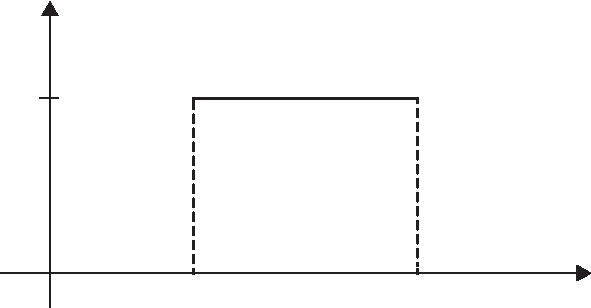
\includegraphics[scale = 0.8]{chapter3/34.pdf}
	\caption{An illustrate of uniform distribution}
\end{figure}

\subsection{10/20 international system}
\hspace{1.5cm} The 10/20 international system is a recognized method to describe and apply the location of scalp electrodes in the context of EEG test. This system is based on the relationship between the location of an electrode and the underlying area of cerebral cortex. The 10/20 international system refers to the actual distance between adjacent electrodes are either 10 \% or 20 \% of the total front-back or right-left distance of the skull. Each site has letters to identify the lobe and a number to identify the hemisphere location. The letters F stands for frontal lobe, T is temporal lobe, C is central lobe, P is parietal lobe, and the last one is O means occipital lobe. Even numbers refer to electrode positions on the right hemisphere and odd numbers refer to the electrode positions on the left hemisphere.

\begin{figure}[h]
	\centering
	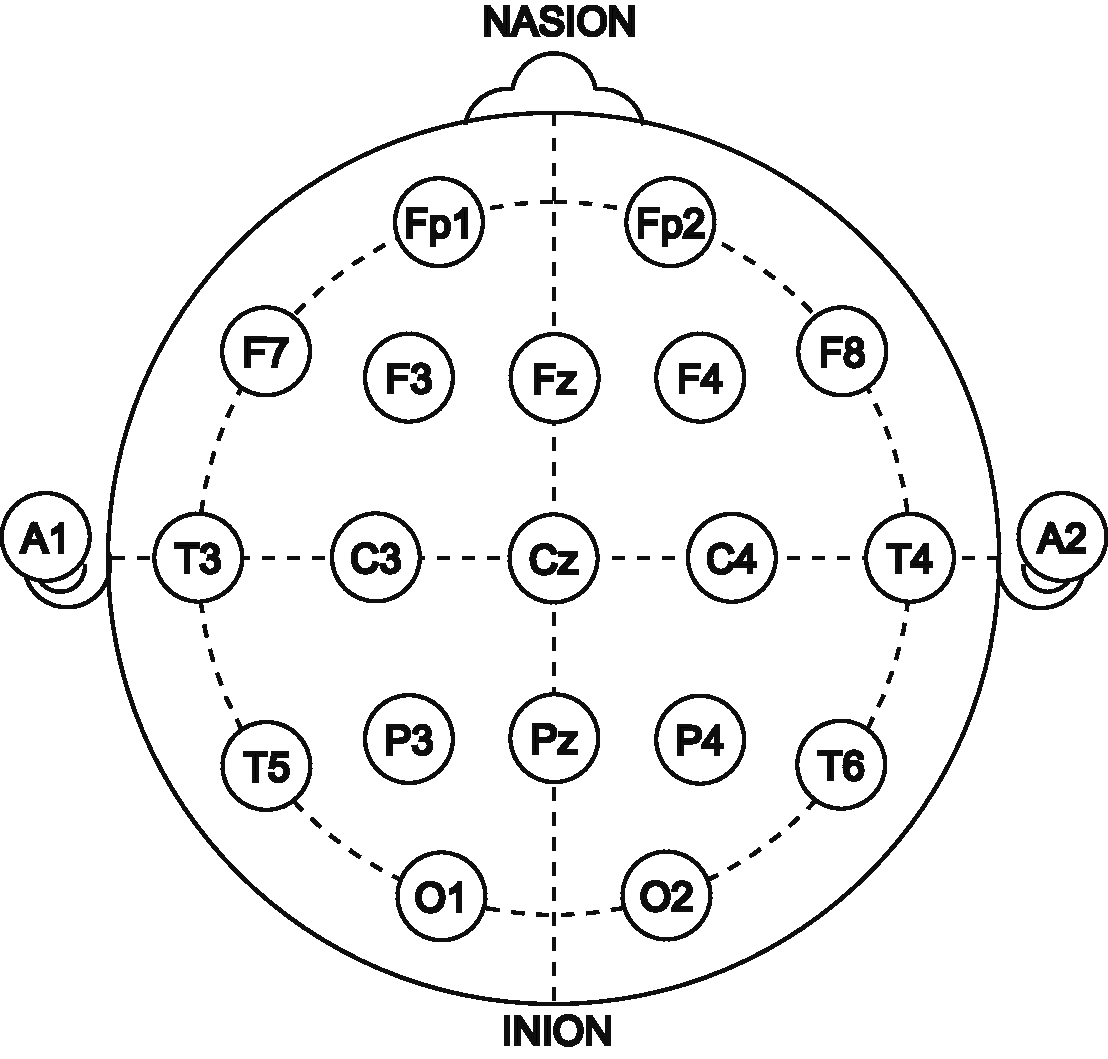
\includegraphics[scale = 0.4]{chapter3/35.pdf}
	\caption{International 10-20 locations system}
\end{figure}

\newpage
\section{Material background}

\subsection{Emotiv EPOC headset\cite{ref12}}

\hspace{1.5cm} The wireless headset Emotiv EPOC research edition, it records EEG data in 14 channel of International 10-20 Locations system with Sequential sampling rate at 128 per second (2048 Hz internal) with resolution 14 bit (16 bit Analog to digital converter, 2-bit instrumental noise floor discarded), the bandwidth is in range 0.2 to 45 Hz with digital notch filters at 50Hz and 60 Hz
\begin{figure}[h]
	\centering
	\includegraphics[scale = 0.01]{chapter3/36.pdf}
	\caption{Emotive Headset}
\end{figure}

\subsection{Gravitech Gerora LED\cite{ref13}}

\hspace{1.5cm} The full colour Light-emitting diode (LED) driver which is use for stimulate the subject has a LED light WS2812 model mounted on. It can chain connected with the same model. It can be controlled by a programmed Arduino. The luminous intensity is 550 to 700 mega candela for red, 1100-1400 mcd for green, and 200-400 mcd for blue.
\begin{figure}[h]
	\centering
	\includegraphics[scale = 0.2]{chapter3/37.pdf}
	\caption{Gravitech Gerora LED base on WS2812}
\end{figure}
\subsection{Arduino UNO\cite{ref14}}

\hspace{1.5cm} The Arduino Uno is a microcontroller board based on the ATmega328 that is an open source platform. It has 14 input/output pins6 analog inputs, a 16 MHz quartz crystal, a USB connection, a power jack, an ICSP header and a reset button, The USB connection for upload the software into the Arduino and VCC or supply for connecting the peripheral circuit.   
\begin{figure}[h]
	\centering
	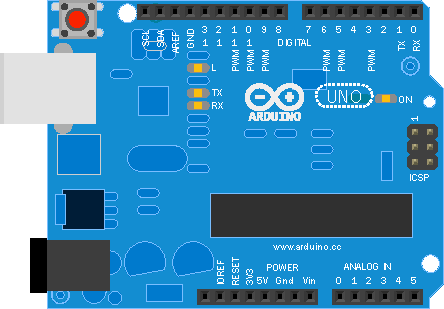
\includegraphics[scale = 0.2]{chapter3/38.pdf}
	\caption{Illustrate of Arduino UNO board}
\end{figure}